% Chapter 3 from the thesis template file
%   that contains an example table and figure.

%Chapter 3 covers the implementation of a Software Defined Radiometer.  It covers how the software defined radio is created in software and compares it to the analog equivilant.  

\chapter{IMPLEMENTATION OF A SOFTWARE DEFINED RADIOMETER}
One of the principal goals with this research was to implement a fully functioning total power radiometer within software.  The N200 provides us the link between the RF signal captured by the antenna and converts that to a format that the computer can now use to manipulate the signal.  Once the signal has been passed to the computer, GNURadio will implement the correct algorithms to detect the power within the signal, filter and output the information.  One of the advantages of course with a SDR is that filtering can also be done within the software.  In addition, thanks to the WxGUI that GNURadio uses, we can also build a user interface that can control several key variables that are useful for us.  This includes controlling the gain on the programmable gain amplifier on the DBSRX2 card, the sampling or bandwidth of the signal, the center frequency, and also the integration time.  All of these can now be controlled in real time as well.  GNURadio will also store the power data so that we are able to do further analysis of the data using a software program like Matlab.  Because GNURadio is a very flexible system we are able to do more with the signal.  We are also able to add additional features and improvements through updates to the software.

\section{Requirements}

Requirements for this system was based on information provided by Dr. Brian Hornbuckle and was also based on requirements of a typical radiometer.  This list is outlined in table~\ref{requirements} shown below.


\begin{table}[h!tb] \centering
\isucaption{ISU Radiometer requirements}
\label{requirements}
\begin{tabular}{lcc} \hline
\textbf{Requirement} & \textbf{Value} & \textbf{Units} \\ \hline
Frequency Range & 1400 - 1420 & MHz \\
Bandwidth & 20 & MHz \\
Polarization & Dual &  \\ 
Sensitivity & -30 & dBm \\
Accuracy & 1 & Kelvin \\ \hline
\end{tabular}
%\vspace{ 2 in}
\end{table}

\subsection{Hardware Requirements}

The selection of the N200 SDR from Ettus Research was based on many of the requirements outlined in table~\ref{requirements}.  In addition, we wanted the hardware to be flexible but also affordable.  There are many different kinds of software defined radios on the market.  However, we choose the N200 based on the availability of the device, the large community support, especially with regards to support by GNURadio, and because it meet and often exceeded the requirements stated above.  

Flexibility was another key aspect of the N200 that made it an excellent selection for this research.  The N200 uses a daughter board setup for bridging the RF interface to the rest of the electronics.  Several different daughter boards are available that have different frequency ranges and offer both receive, transmit and transceiver designs.  For the radiometer we need to operate around 1.4 GHz and receive only.  Based on those requirements we choose the DBSRX2 daughter board.  This board is designed from 800 MHz to 2.3 GHz and has a fairly low noise figure.   

The current RF front end to the radiometer is designed for a 20 MHz wide signal.  This requirement was one of the main driving points for selecting the N200 SDR as it can support up to 50 MHz in bandwidth between the N200 and the host computer.  This is accomplished by using a 1 Gbps Ethernet connection between the N200 and the host computer.

\subsection{Software Requirements}

The driving force for the software requirement was to have a system that was easy to use yet powerful enough to handle the amount of data that is required.  One reason for the development of this platform is to make radiometers more accessible to other researchers and other programs such as education and even amateur radiometer work.  Therefore ease of use was taken into consideration when selecting the hardware and the associated software used with it.

The data flow model for the hardware selected uses the FPGA to perform low level signal processing on the signal and moves high level processing to the host computer.  This allows for less processing requirements on the physical hardware but requires a host computer that is able to process the incoming information.  It also requires a software package that is able to process this information efficiently. 

Because a requirement is an easy to use system GNURadio was selected as it includes GNURadio Companion (GRC). GRC is a supplemental program which uses a graphical interface for creating the radio environment.  It also includes options to create a user interface during the operation of the N200 as well.  This allowed us to rapidly create both the critical radio components needed for the radiometer and also a control interface.

This software meet the criteria of allowing a simple to use interface to be built and used in the control and data recording of the information required.  It also uses a simple interface for making changes to the program.  These changes can be both in the GUI and also to how the program processes the information.

\section{Power detection}
Power detection is a key ability that allows a radiometer to function.  At its core a radiometer is a power detector.  Therefore the implementation of power detection is a crucial function of a software defined radio radiometer.

To implement a total power radiometer in software we first need to look at how we implement a total power radiometer traditionally.  Traditionally, a square law detector is used to detect the average power that is seen by the radiometer.  This simple device uses a diode that gives a small voltage output based on the RF power present.  This small voltage is then amplified and can now be calibrated with a known source to give us a noise temperature.  

{\begin{figure}[h!tb] 
\centering
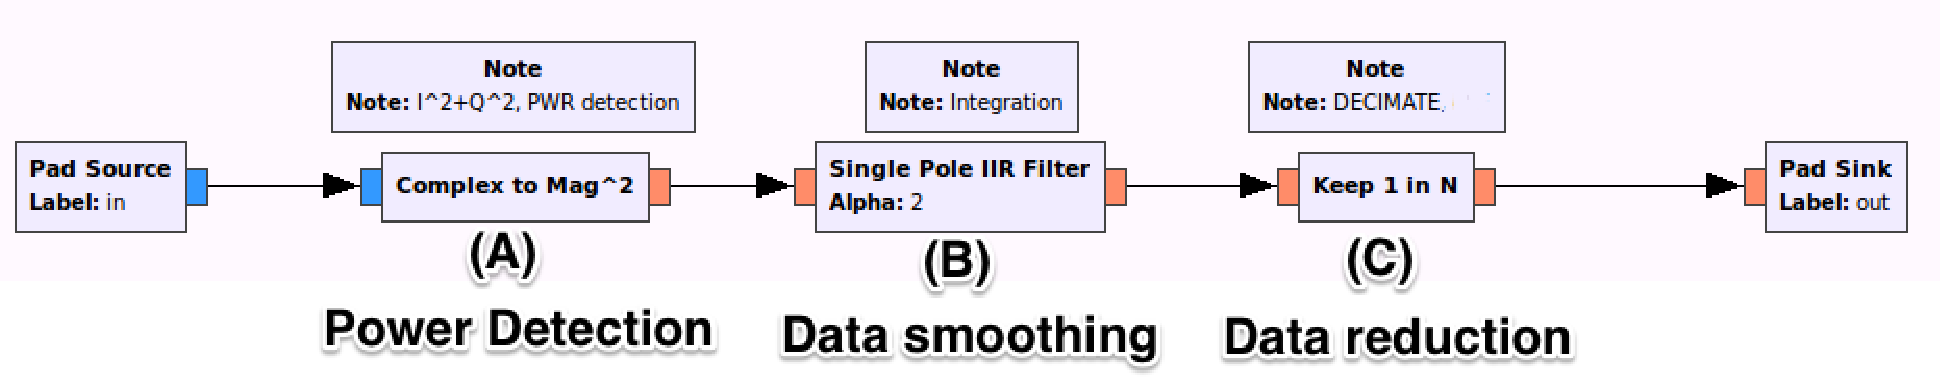
\includegraphics[width=17cm]{Images/TPR_grc.png}
\isucaption{A block diagram showing how the radiometer performs the equivalent square law detector in software.}
\label{square_block}
\end{figure}
}

To implement this in software we need to build a square law detector mathematically.  We can then give this to the software defined radio to process the information accordingly.  A square law detector mathematically is the sum of the squares.  Once the signal has been digitized, it is expressed in data bits of I and Q, which represent in-phase and quadrature-phase of the signal.  By squaring each term, we get the desired result of the power of the signal [\cite{Sarijari}][\cite{Rashid}] can be shown in equation \ref{sdr_x2}.

\section{Integrator through a IIR Filter}

Another step that we typically do in a traditional radiometer is to integrate the signal over time.  This gives us an average of the signal and smooths out the output.  In addition, we will show later that the integration time can be adjusted to help improve our sensitivity of the radiometer.

In a traditional radiometer, we can integrate by using a simple integrator circuit, which consists of an op-amp, resistor and capacitor.  This circuit configuration is also equivalent to a low pass filter circuit as well, and the two are interchangeable.  We can then look at how we filter in the digital domain, and this is down with a infinite impulse response filter or IIR.  We can use this digital filter to then integrate the signal for our total power radiometer. Again, this relationship between the IIR filter and the integrator is explained in chapter 2 and is mathematically shown in equation \ref{final_IIR_RC}.

\section{GNURadio Blocks}
A software defined radio by its definition requires software for the proper operation of the radio.  In our case there is the software or firmware that resides on the FPGA and then the software that runs on the computer.  For this thesis, we focused on the software running on GNURadio.  This software package provides us with the ability to write the code needed to implement a total power radiometer but also gives us a method to control the SDR as well.  It also allows for us to record the information for performing post-processing on the data.

\section{Control of the SDR Hardware through GNURadio}
The N200 sends all data across the 1 Gbps connection to be read in by a host computer running GNURadio.  This data is the raw I/Q values that is read by the on board A/D and processed by the on board FPGA.  An example of a very simple GNURadio software implementation would simply take this data and store the data to a hard drive in a file.  This can be very handy if we want to simply record the data and then process it later.  However, depending on the sample rate, it can consume a large amount of storage.  A short recording can easily consume 1-2 GB with a sample rate of 10 Msps.  It also does not give us any immediate feedback on the radiometer and it does not give us controls of the radiometer such as frequency, integration time or other key variables.  Fortunately GNURadio has tools that allows us to build up a very rich application that is able to give us the data we need and control the software defined radio as well.

The GNURadio Companion allows us to create python code that is used to not only receive the data from the SDR but also perform signal processing on the incoming information.  Additional controls are added that allow for tuning of the signal processing parameters and control of the radio functions.  This allows us to build up an application that can be run on any computer that is capable of running GNURadio.  

{\begin{figure}[h!tb] 
\centering
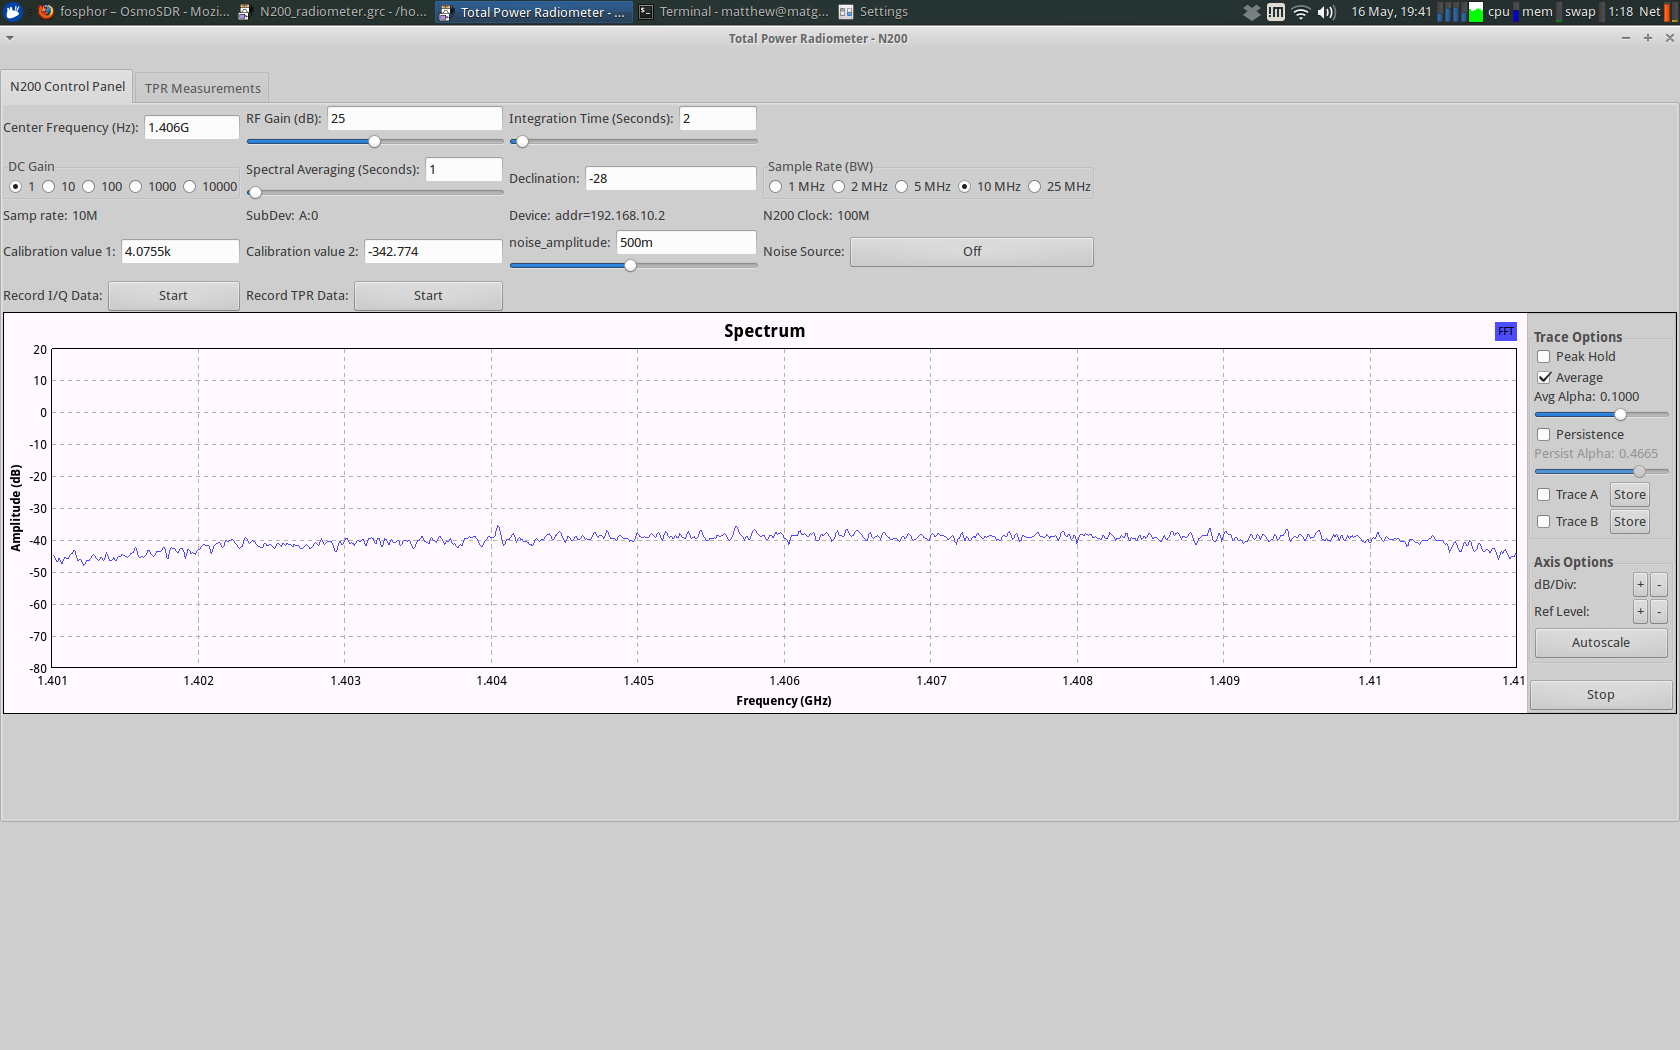
\includegraphics[width=17cm]{Images/radiometer_gui.png}
\isucaption{A screenshot of the interface made for communication with and controlling the software defined radio}
\label{radiometer_gui}
\end{figure}
}

Through this interface we are able to control several key aspects of not only the radio hardware within the SDR but also with the behavior of the radiometer as well.  Hardware control of the SDR hardware allows us to change frequency and also adjust gain values within the N200.  Bandwidth is another parameter that can be altered from here as well.  Bandwidth affects the bandwidth for the RF signal, but also has an impact on the radiometer sensitivity as well.  Additional controls allows for alterations to the radiometer and includes being able to adjust the integration time of the radiometer.  

\subsection{Impact of the Controls Related to Radiometry}

The controls that have been added for controlling the radiometer can have a large impact on the performance of the radiometer.  There is a reason why these controls were added to the GUI for the radiometer and that is they play key roles in how the radiometer performs.  

For any radiometer noise temperature is a large consideration and is critical to the design of the radiometer.  One method to determine how well a radiometer is to look at the sensitivity of the radiometer.  We can do this by looking at the smallest change in temperature the radiometer can see.  We will call this the Noise Equivalent $\Delta T$ or $NE\Delta T$ of the radiometer.  The equation for this is shown below.

\begin{equation}
NE\Delta T=\frac{T_{A}+T_{sys}}{\sqrt{\beta * \tau}}
\end{equation}

$\beta$ can be changed by changing the sample rate of the SDR.  The sample effectively controls the bandwidth in which the SDR is operating at.  This also gives us a band-pass filter as well, since the SDR will not respond to frequencies outside of this bandwidth.  

$\tau$ is the integration time for the radiometer.  This parameter is set by the user through the GUI and allows us to change the integration time in seconds.

\section{GNURadio Data Handling}
Once we have the data that has been processed by the software defined radio we will want to display this information and be able to store the data so we can analyze it later if needed.  Data display can be handled GNURadio where we can plot the total power over time.  This allows the user to be able to visualize the total power and be able to determine if the total power has increased or decreased over the time window shown.  

Although not usually needed for a total power radiometer we also have the ability to look at the signal in terms of a frequency versus amplitude.  This allows to look for any unusual signals that may be interfering with or causing erroneous data with our radiometer.  

Finally we will want to store the data so we can do additional analyses on it at a later time.  The GNURadio program allows us to store the data in two formats.  The first format is storing the raw I/Q data from the radiometer.  This format allows us to "playback" the data through GNURadio at a later time.  This can be useful for if we wish to change parameters in GNURadio such as bandwidth or integration time.  It is also a good diagnostic tool as we can check that the signal coming in is clean or if we need to apply additional filters to remove an unwanted signal. This file may be quite large, consuming several gigabytes of data for a 20 MHz wide signal in a matter of minutes of record time.

The second format is the total power that has been calculated by the radiometer.  This file is much smaller in size since much of the signal information has now been reduced to simple power versus time information.  This allows for easy manipulation through any math program such as Matlab for analysis.  

\subsection{GNURadio Data Display}
The information from the software defined radio can be displayed through GNURadio to show a number of things.  Since we have both frequency and magnitude information we can display this information.  We are able to also display the information that shows the total power that is being seen by the radiometer as well.

{\begin{figure}[h!tb] 
\centering
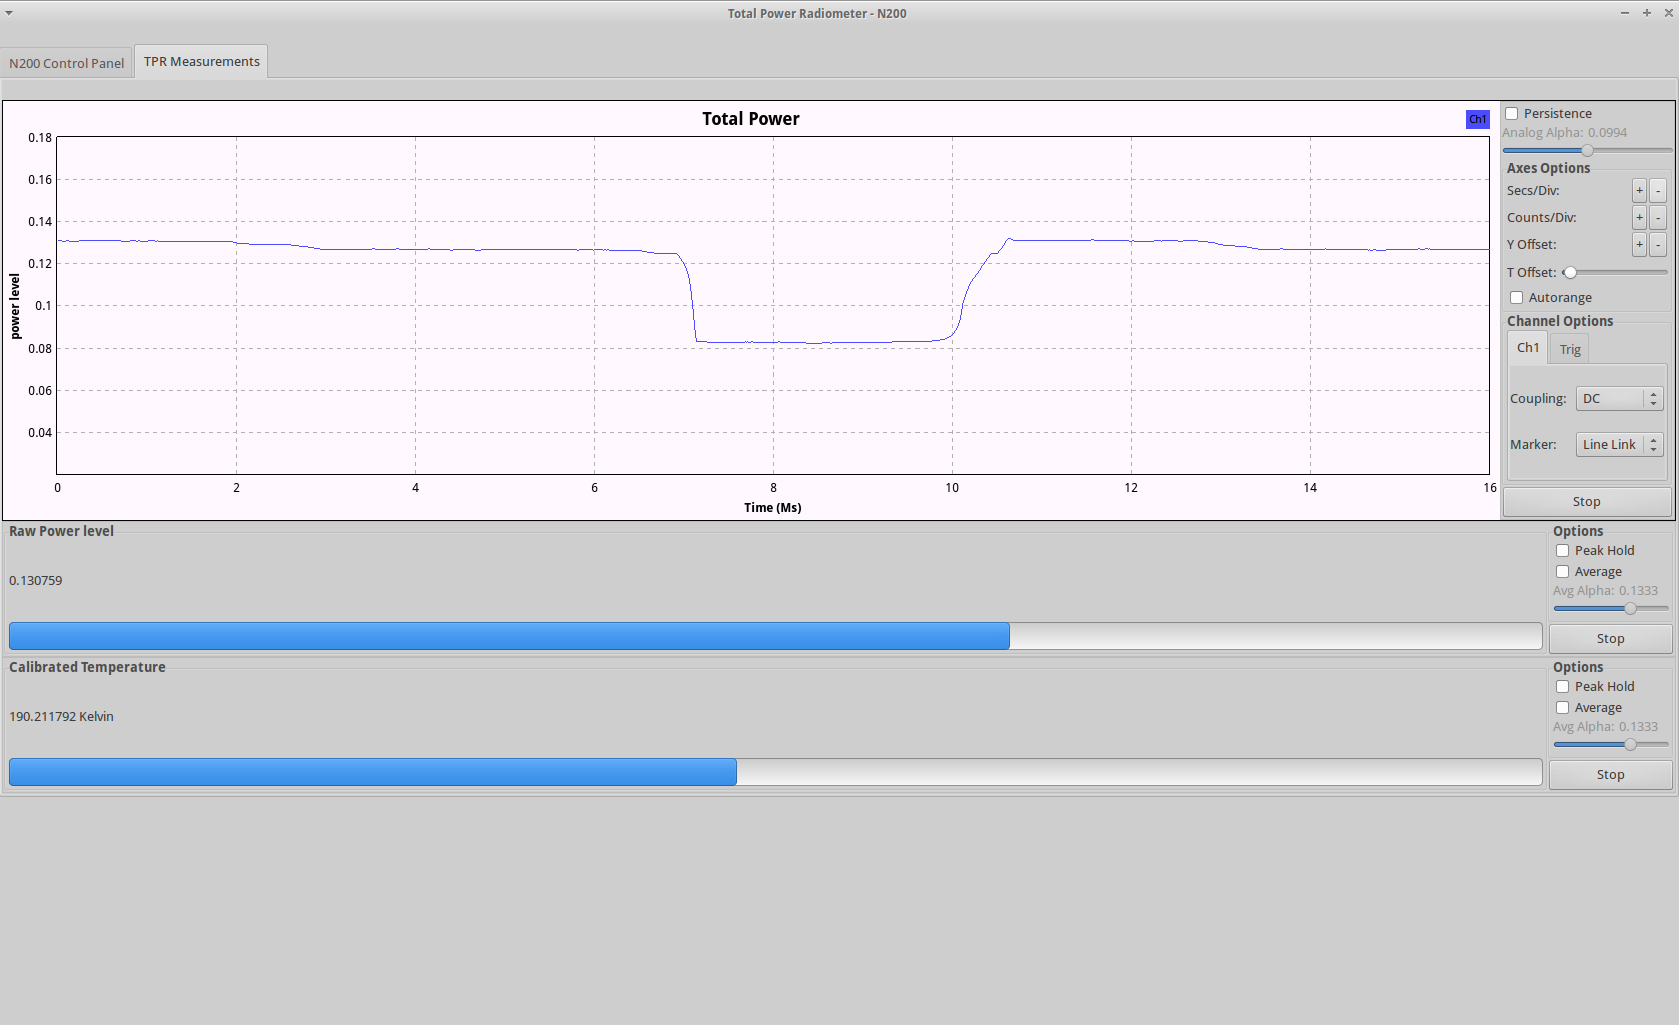
\includegraphics[width=17cm]{Images/Lab1_TPR_at_end_exp.png}
\isucaption{A screenshot showing the ticker tape display for the total power readings.  In addition raw and calibrated noise temperature is shown below.}
\label{radiometer_tpr_display}
\end{figure}
}

We are not limited to just total power from the radiometer.  If the radiometer has been calibrated, those calibration points can be entered and GNURadio can calculate the calibrated noise temperature.  Additional information may also be added as needed.  For example, we are able to view the full spectrum that the radiometer sees.  This can be a useful tool for looking at potential RFI issues.    

\subsection{GNURadio Data Processing}

GNURadio is capable of storing information in files that can be processed later.  These files are binary formats that are stored in a little-endian format and can be a character, integer, float or complex.  A simple example is storing the raw I/Q values to a file.  This file can then be processed by Python, GNURadio, or even Matlab.  For example, we can store the raw I/Q values and then play them back though GNURadio.  Of course other information can be stored as well and we use this same method to store the total power radio values to a file as well.  

{\begin{figure}[h!tb] 
\centering
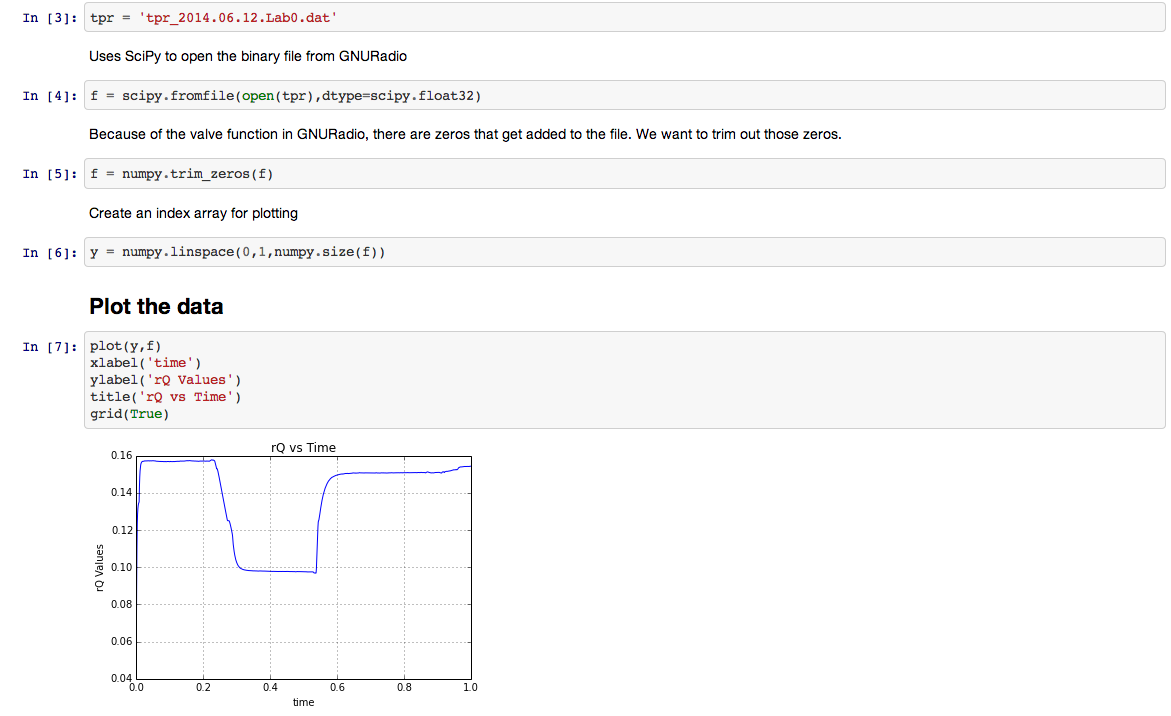
\includegraphics[width=17cm]{Images/python_gnuradio.png}
\isucaption{A screenshot showing the iPython notebook code and related graphs generated for parsing GNURadio data}
\label{matlab_display}
\end{figure}
}

Matlab is one tool we can use to process the information that is stored by GNURadio.  Appendix A contains the Matlab source that will read the total power file generated by GNURadio.  It then calculates information such as the NE$\Delta$T and the calibration points based on the user input.  We can also use Matalb to graph this information as well.

While Matlab is one tool, other tools can be used.  Python for example is also capable of reading in these files and when paired with NumPy and SciPy can be used to perform analysis on the data as well.  In addition, the open source mathematical program Octave should also be able to read and work with these files.  For this thesis both Matlab and Python was used to provide analysis on the data.  

Most of the graphs generated in this thesis was generated using iPython notebooks.  iPython notebooks uses Python but allows it be executed in a web browser either locally or on a server.  Using iPython notebooks however also allows us to add additional information using Markdown and basic HTML.  This allowed the author to paint a complete picture of the experimental results illustrating pictures of the setup and the code and steps used to analyze the data.  You can find these notebooks on the author's Github site and can use NBViewer to view them.  An example link is \href{http://nbviewer.ipython.org/github/matgyver/Radiometer-SDR-Thesis/blob/master/Experiments/Exp1/radiometer_experiment_1.ipynb}.
